\begin{frame}[allowframebreaks]{Unsupervised Learning - Applications}
    Deep Unsupervised Learning has many powerful applications:
    \begin{itemize}
        \item \textbf{Generate Novel Data}: Create new data samples similar to the training set.
        \item \textbf{Conditional Synthesis Technology}: Enable advanced applications such as WaveNet for audio generation and GAN-based models like pix2pix for image-to-image translation.
        \item \textbf{Compression}: Learn compact representations for efficient data storage and transmission.
        \item \textbf{Improve Downstream Tasks}: Enhance performance of supervised tasks through unsupervised or self-supervised pre-training.
        \item \textbf{Production-Level Impact}: Power real-world systems, e.g., Google Search improvements with BERT pre-training.
        \item \textbf{Flexible Building Blocks}: Provide reusable components for a wide range of machine learning pipelines.
    \end{itemize}
\end{frame}

\begin{frame}[allowframebreaks]{Application: Generate Images}
    \begin{figure}
    \centering
    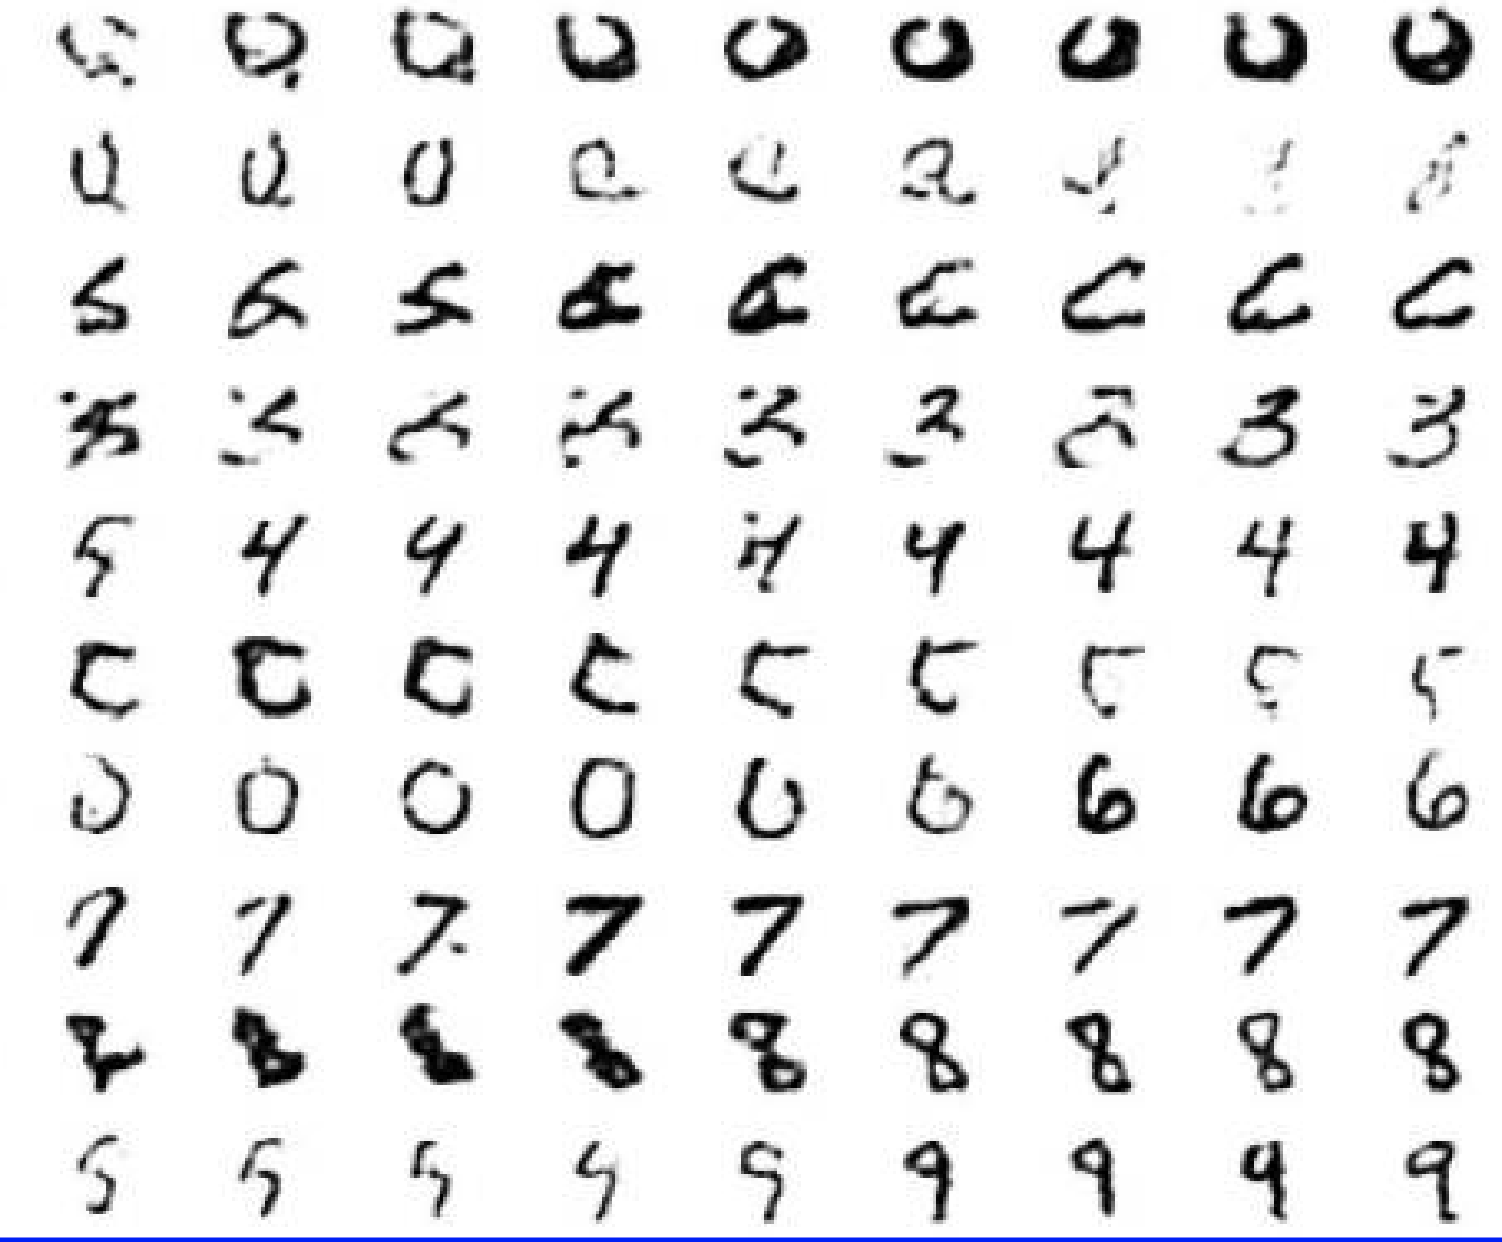
\includegraphics[height=0.8\textheight]{images/dul/slide_19_1_img.png}
    \caption{[Deep Belief Nets, Hinton, Osindero, Teh, 2006]}
    \end{figure}

    \framebreak

    \begin{columns}
        \column{0.5\textwidth}
            \begin{figure}
                \centering
                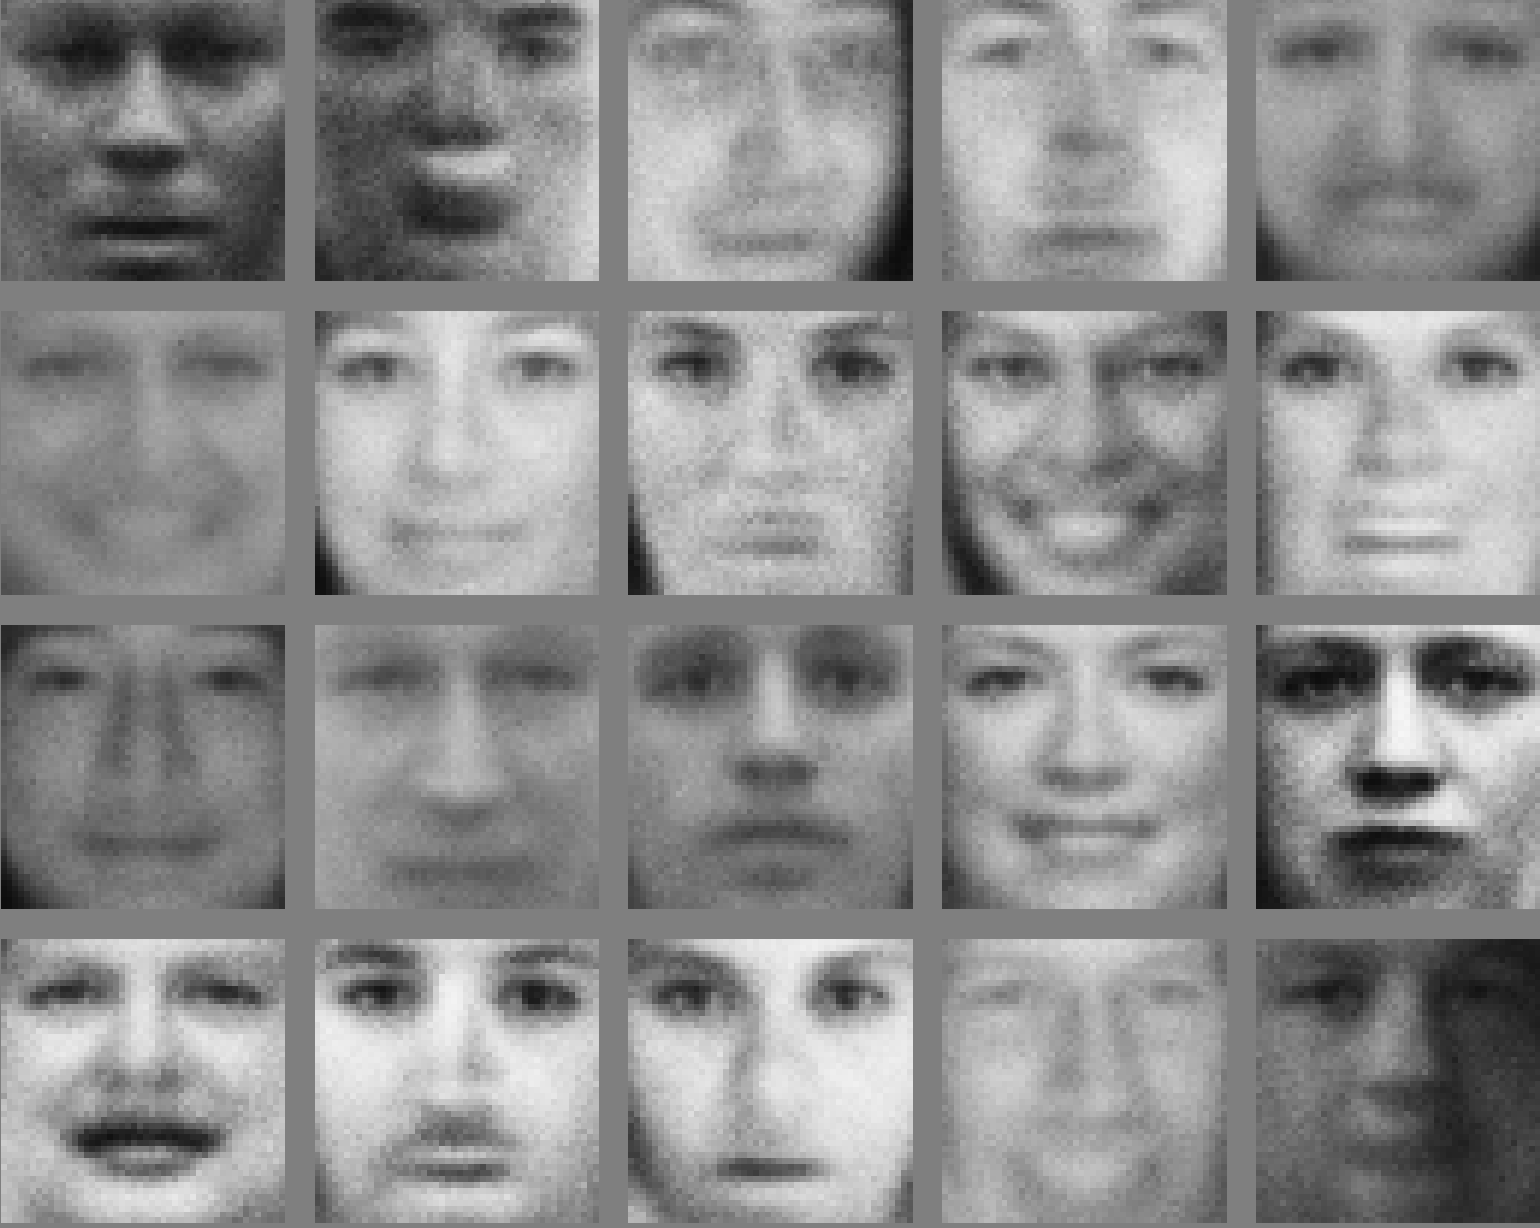
\includegraphics[width=1\textwidth]{images/dul/slide_21_1_img.png}
            \end{figure}
        \column{0.5\textwidth}
            \begin{figure}
                \centering
                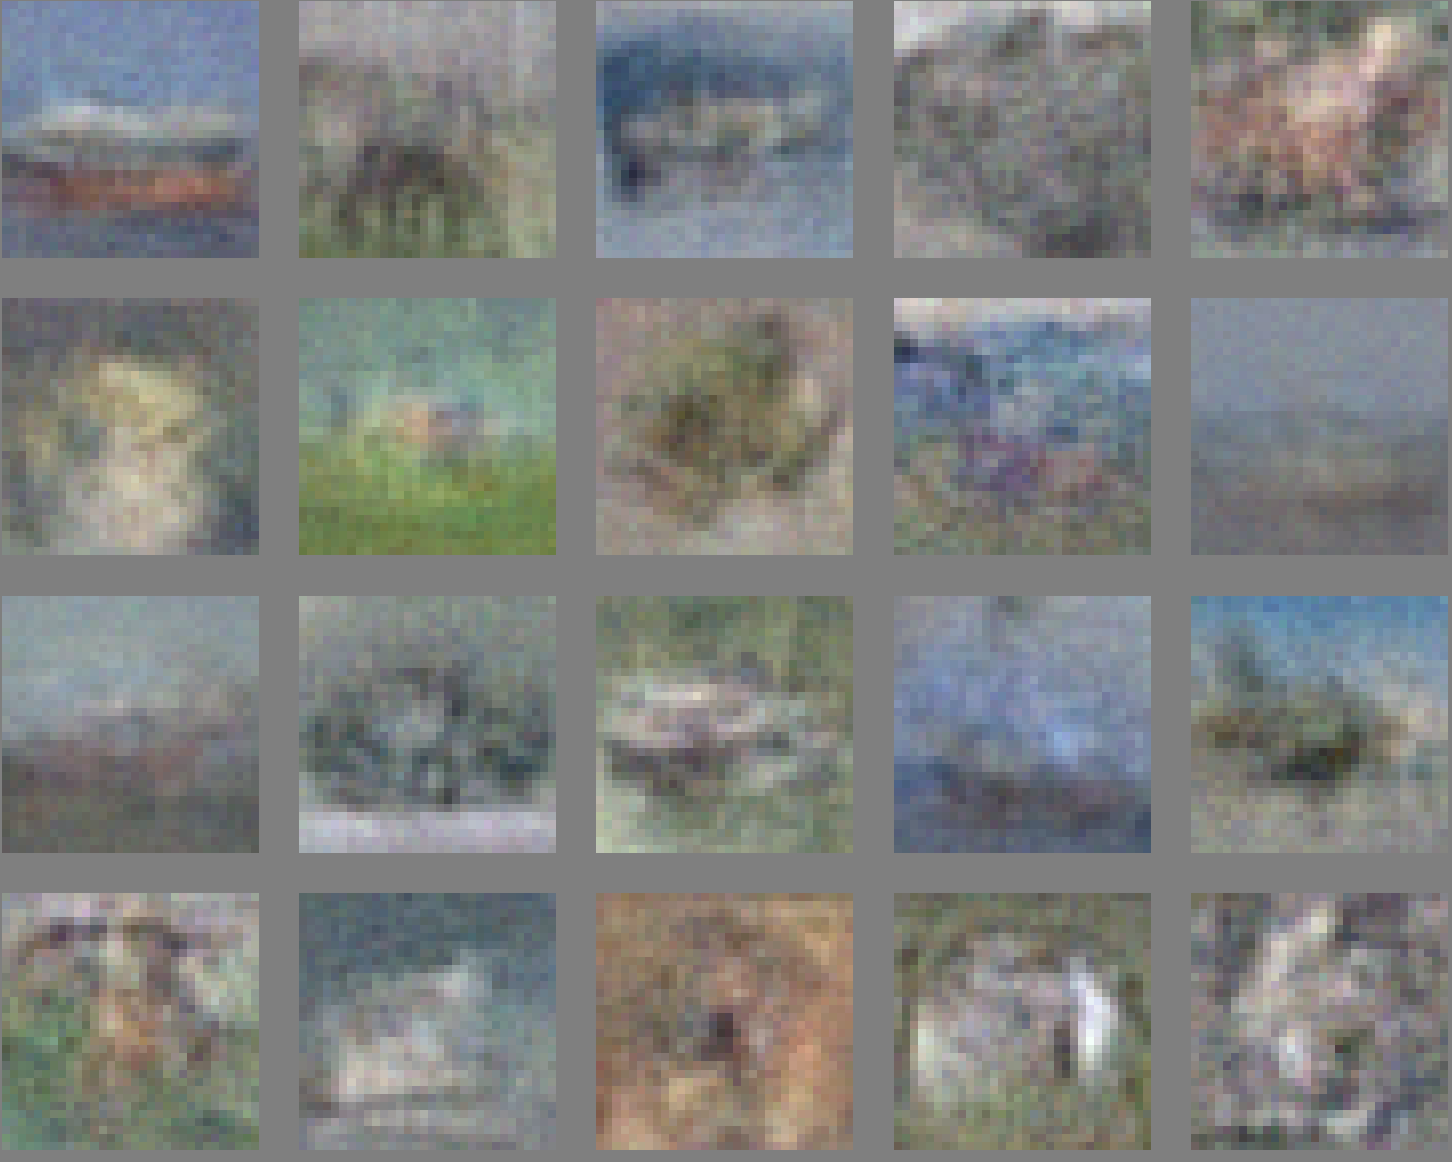
\includegraphics[width=1\textwidth]{images/dul/slide_21_2_img.png}
            \end{figure}
    \end{columns}
    \vspace{1em}
    \centering
    [GAN, Goodfellow et al. 2014]

\end{frame}


\begin{frame}{Application: Discovering Structure in Digits}
    \begin{figure}
    \centering
    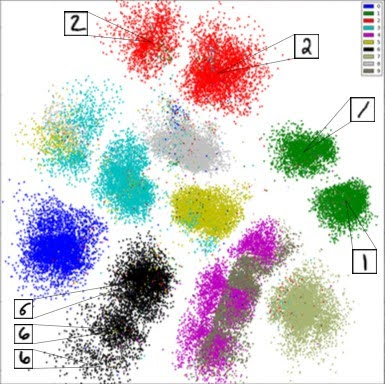
\includegraphics[width=0.8\textwidth,height=0.75\textheight,keepaspectratio]{images/dul/discover-structure.jpg}
    \caption{Unsupervised learning can discover structure in digits without any labels.}
    \end{figure}
\end{frame}

\begin{frame}{Application: DNA Analysis}
    \begin{figure}
    \centering
    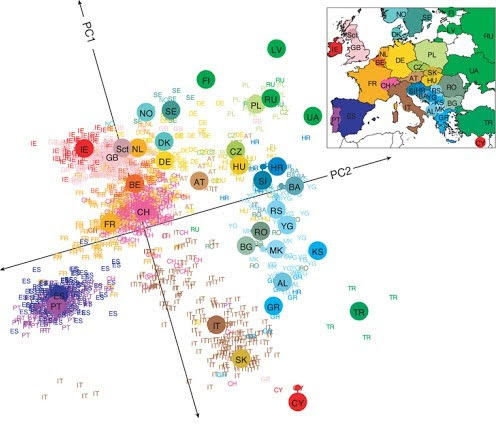
\includegraphics[width=0.8\textwidth,height=0.75\textheight,keepaspectratio]{images/dul/dim-reduce.jpg}
    \caption{Dimensionality reduction applied to DNA reveal the geography of European countries.}
    \end{figure}
\end{frame}

\begin{frame}{Application: Text to Image Generation}
    \centering
    “a masterful oil painting a persian exotic cat discovering their astounding crypto losses while checking their phone”
    \begin{figure}
    \centering
    
\includegraphics[width=0.8\textwidth,height=0.75\textheight,keepaspectratio]{images/dul/slide_29_1_img.png}
    \end{figure}
\end{frame}

\begin{frame}[allowframebreaks]{Application: Text to Audio Generation}
    \begin{figure}
    \centering
    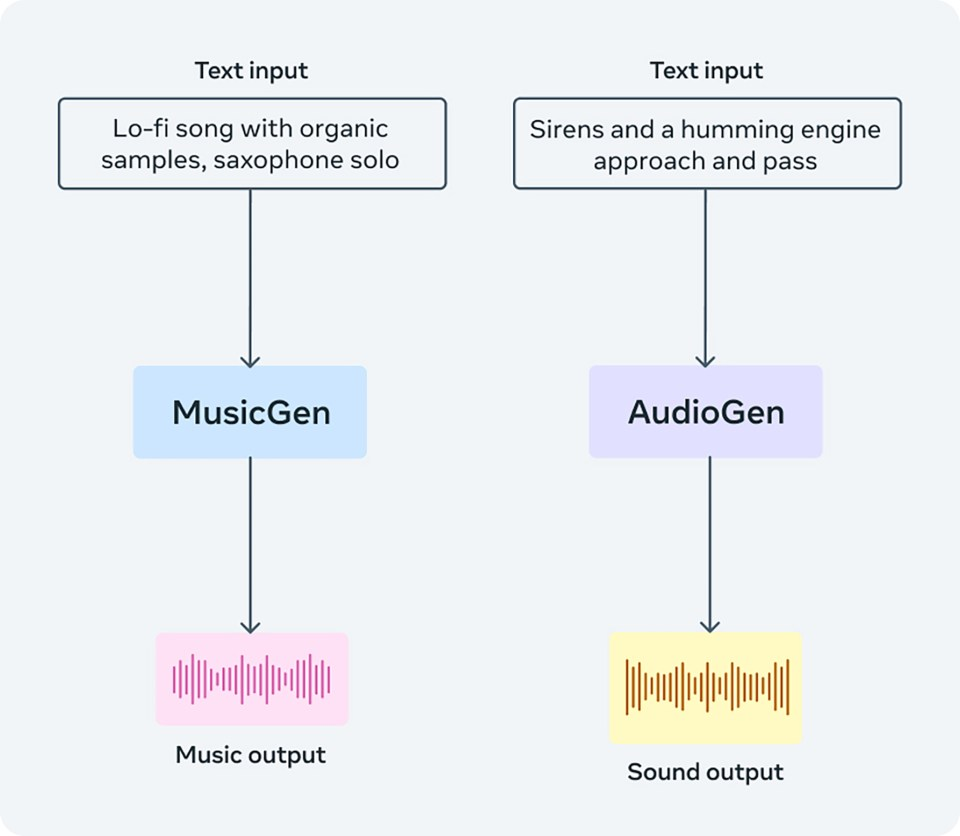
\includegraphics[height=0.8\textheight]{images/dul/slide_34_1_img.png}
    \caption{[AudioCraft, Copet et al., 2023]}
    \end{figure}
\end{frame}

\begin{frame}[allowframebreaks]{Application: Text to Speech Generation}
    \begin{figure}
    \centering
    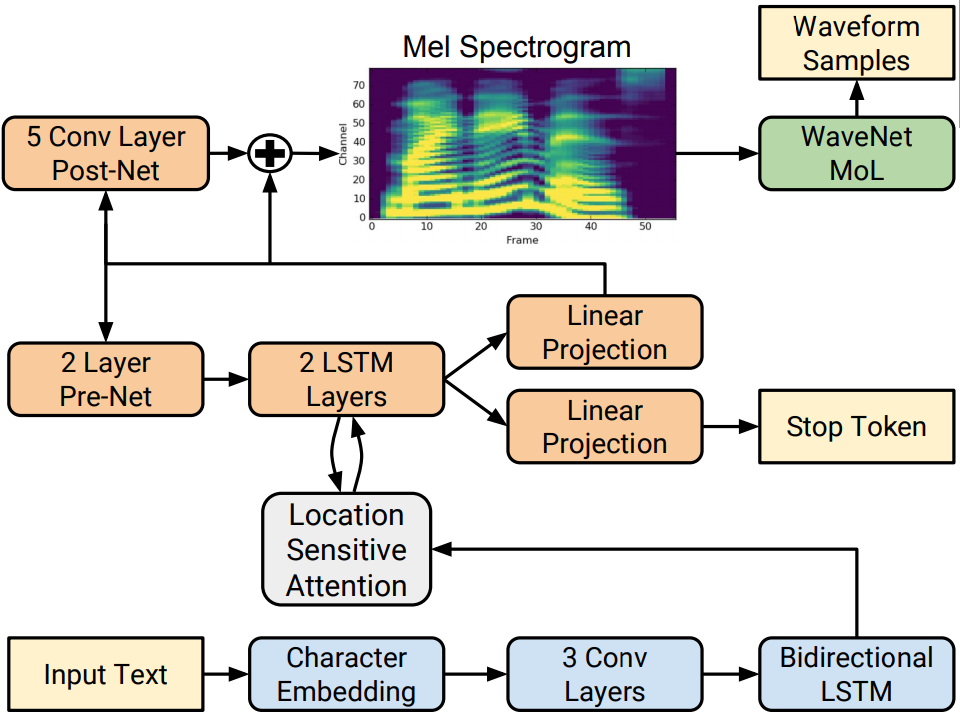
\includegraphics[height=0.8\textheight]{images/dul/slide_35_1_img.png}
    \caption{[Tacotron2 , Shen et al., 2018]}
    \end{figure}
\end{frame}

\begin{frame}[allowframebreaks]{Application: Generate Math}
    \begin{figure}
    \centering
    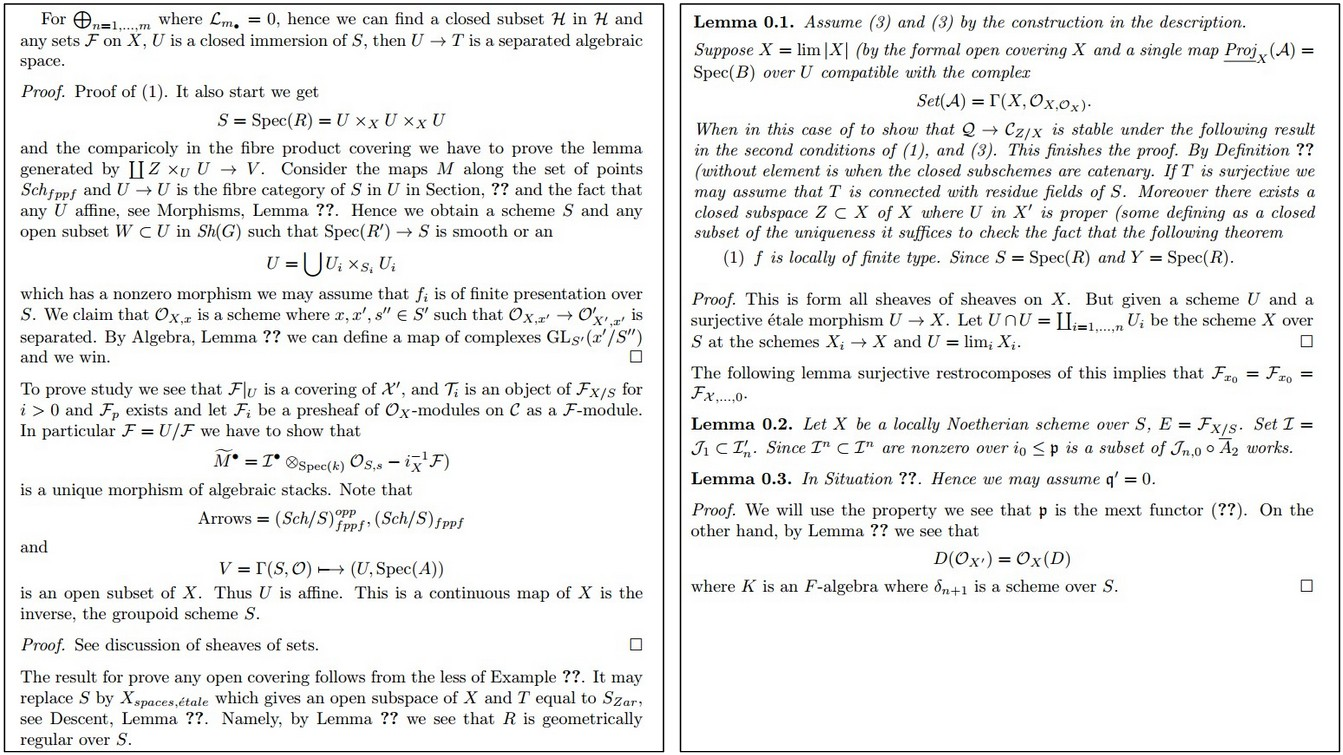
\includegraphics[height=0.8\textheight]{images/dul/slide_43_1_img.png}
    \caption{[Char-rnn, karpathy, 2015]}
    \end{figure}
\end{frame}

\begin{frame}[t]{Application: Generate Text}
    \textbf{Prompt [human written]}: 
    {\small A train carriage containing controlled nuclear materials was stolen in Cincinnati today. Its whereabouts are unknown.} \\
\textbf{GPT-2}: {\small The incident occurred on the downtown train line, which runs from Covington and Ashland stations. In an email to Ohio news outlets, the U.S. Department of Energy said it is working with the Federal Railroad Administration to find the thief.
‘The theft of this nuclear material will have significant negative consequences on public and environmental health, our workforce and the economy of our nation,’ said Tom Hicks, the U.S. Energy Secretary, in a statement. ‘Our top priority is to secure the theft and ensure it doesn’t happen again.’
The stolen material was taken from the University of Cincinnati’s Research Triangle Park nuclear research site, according to a news release from Department officials.
The Nuclear Regulatory Commission did not immediately release any information. According to the release, the U.S. Department of Energy’s Office of Nuclear Material Safety and Security is leading that team’s investigation.
‘The safety of people, the environment and the nation’s nuclear stockpile is our highest priority,’ Hicks said. ‘We will get to the bottom of this and make no excuses.’}

\vspace{0.25em}
\centering
{\small[OpenAI’s GPT2 -- Radford, Wu, Child, Luan, Amodei, Sutskever, 2019]}
\end{frame}